\chapter{التطور الجزيئي والجينوميات التطورية}\label{ch:b3:molecular-evolution}

في عام 1968 أجرى موتو كيمورا حسابًا أقلق حقلًا بأسره. فبمقارنة
الهيموغلوبينات والسيتوكرومات وغيرها من بروتينات ثدييات
أُرِّخت أسلافها المشتركة بالأحافير، وجد أن الأحماض الأمينية
استُبدلت بمعدل يقارب استبدالًا واحدًا لكل موقع في كل مليار
سنة --- وهو ما يبلغ، على جينوم ثديي وجيل واحد، استبدالًا
جديدًا يتثبت في الجمهرة كل سنتين أو نحوهما. وكان هالدين قد
بيّن قبل عقد أن الانتخاب الطبيعي لا يقدر على تثبيت أكثر من
استبدال واحد كل ثلاثمئة جيل تقريبًا قبل أن تصير الكلفة في
الخلف الضائع غير قابلة للدفع. فلم يترك الحساب إلا مخرجًا
واحدًا: أن معظم التغيّرات التي تتراكم في DNA لا يسوقها
الانتخاب البتة، بل هي محايدة، تُثبَّت بالمصادفة في جمهرات
منتهية، بمعدل هو --- كما تبيّن مبرهنة هذا الفصل الأولى ---
معدل الطفر نفسه. وصارت \omterm{thm:b3:molecular-evolution:neutral}{النظرية المحايدة} فرضية العدم في
التطور الجزيئي، وخط الأساس الذي يُكشف الانتخاب في مواجهته؛
وصارت \omterm{prop:b3:molecular-evolution:clock}{الساعة الجزيئية} طريقة لتأريخ ما لا تقدر الأحافير على
تأريخه؛ وأعطت الجينومات المسلسلة منذ ذلك الحين أدوات لرؤية،
مورّثةً مورّثة، أين عمل الانتخاب، وكيف تولد مورّثات جديدة من
قديمة، ولماذا لا تكون \omterm{prop:b3:molecular-evolution:ils}{شجرة المورّثة} دائمًا شجرة نوعها.

\section{الانجراف، والطفر، والمعدل المحايد}

\begin{theorem}[معدل الاستبدال المحايد]\label{thm:b3:molecular-evolution:neutral}
\index{نظرية محايدة}\index{معدل الاستبدال}\index{احتمال التثبّت}\index{انجراف وراثي}
في جمهرة ثنائية الصيغة من $N$ فرد، تكون لطفرة جديدة لا أثر
لها في الملاءمة احتمال $1/2N$ أن تحل في النهاية محل كل
الأليلات الأخرى (\emph{التثبّت}) واحتمال $1 - 1/2N$ أن تضيع.
وإذا طفرت كل نسخة من نسخ المورّثة $2N$ بمعدل $\mu$ في الجيل،
نشأت $2N\mu$ طفرة محايدة جديدة في الجيل، وكان المعدل الذي
تتراكم به الاستبدالات على المدى الطويل
\[
k = 2N\mu\times\frac{1}{2N} = \mu :
\]
أي إن \emph{\omterm{thm:b3:molecular-evolution:neutral}{معدل الاستبدال}} المحايد يساوي معدل الطفر، مستقلًا
عن حجم الجمهرة. والطفرة المقدَّر لها أن تتثبت تستغرق وسطيًا
$4N$ جيل لتفعل، فتحمل الجمهرات الكبيرة تباينًا أكثر في
الطريق لكنها لا تثبّته أسرع. وأما الطفرة ذات الأفضلية
الانتخابية $s$، فتعطي صيغة كيمورا \omterm{thm:b3:molecular-evolution:neutral}{احتمال التثبّت}
\[
P(s) = \frac{1 - \mathrm{e}^{-2s}}{1 - \mathrm{e}^{-4Ns}} \approx 2s
\quad (4Ns \gg 1),
\]
فتُثبَّت أفضلية قدرها \qty{1}{\%} باحتمال نحو
\qty{2}{\%} --- أي أربعين ضعف حظ طفرة محايدة في
جمهرة من ألفين، ومع ذلك تضيع تسعًا وأربعين مرة من كل خمسين؛
وأما مساوئ $s < 0$ عند $4N|s| \gg 1$ فلا تُثبَّت أبدًا
تقريبًا، وأما التي عند $4N|s| \ll 1$ فتسلك سلوك المحايدة:
فالانتخاب لا يرى إلا ما لا يغرقه الانجراف، والحد $|s| \sim
1/4N$ --- أي \emph{المحايدة فعليًا}.
\end{theorem}
\begin{proof}
أما الحياد: فنسخة ما حاضرة اليوم ستكون سلفًا للجمهرة كلها في
المستقبل البعيد، وبالتناظر يكون احتمال أن تكون كلُّ نسخة من
النسخ $2N$ هي تلك النسخةَ متساويًا؛ والطافرة الجديدة نسخة
واحدة، فيكون $1/2N$. وأما المعدل: فالاستبدالات في الجيل $=$
(الطفرات الناشئة في الجيل) $\times$ (احتمال تثبّت كل واحدة)
$= 2N\mu/2N$. وصيغة كيمورا تتبع من تقريب الانتشار لتغيّر تواتر
الأليل تحت الانجراف والانتخاب، وهو مُسلَّم به هنا؛ وتُتحقَّق
حدودها مباشرةً: فحين $s \to 0$ يكون $(2s)/(4Ns) = 1/2N$، وهي
القيمة المحايدة؛ وعند $4Ns \gg 1$ يكون المقام $1$ والبسط
$\approx 2s$. وأما زمن التثبّت: فتواتر أليل محايد يؤدي مشيًا
عشوائيًا بتباين $p(1-p)/2N$ في الجيل، والزمن المتوقع لبلوغ
$1$ من $1/2N$، بشرط بلوغه، هو $4N$ جيل (كيمورا وأوتا، 1969)،
وهو مُسلَّم به.
\end{proof}

\begin{omfigure}
\begin{tikzpicture}
\begin{semilogyaxis}[
  width=0.62\linewidth, height=5.6cm,
  axis x line=bottom, axis y line=left,
  xmin=-4, xmax=8, ymin=0.00002, ymax=0.2,
  xlabel={$4Ns$ (معامل الانتخاب المدرَّج)}, ylabel={احتمال التثبّت},
  xlabel style={font=\small, at={(axis description cs:0.5,-0.12)}, anchor=north}, ylabel style={font=\small},
  tick label style={font=\small}, xtick={-4,-2,0,2,4,6,8}, ytick={0.0001,0.001,0.01,0.1}, yticklabels={$10^{-4}$,$10^{-3}$,$10^{-2}$,$10^{-1}$},
  clip=false,
]
\addplot[very thick, omDef, domain=-4:-0.05, samples=60] {(x/2000)/(1-exp(-x))};
\addplot[very thick, omDef, domain=0.05:8, samples=80] {(x/2000)/(1-exp(-x))};
\draw[dashed, gray] (axis cs:-4,0.0005) -- (axis cs:8,0.0005); \node[font=\scriptsize, gray, anchor=north west] at (axis cs:-3.9,0.00048) {محايد، $1/2N$};
\addplot[thick, omThm, dashed, domain=1:8, samples=2] {2*x/(4*1000)};
\node[font=\scriptsize, omThm, anchor=north west] at (axis cs:5,0.0012) {المقارب $2s$};
\node[font=\scriptsize, omDef, anchor=south east, align=right] at (axis cs:-0.2,0.02) {محايد فعليًا\\حين $|4Ns| \lesssim 1$};
\node[font=\scriptsize, omDef, anchor=south west] at (axis cs:-3.9,0.0008) {ضار: لا يتثبت أبدًا تقريبًا};
\end{semilogyaxis}
\end{tikzpicture}

{\small \omterm{thm:b3:molecular-evolution:neutral}{احتمال التثبّت} عند كيمورا في مقابل معامل الانتخاب
المدرَّج، عند $N = 1000$. فقرب الصفر يمر المنحني بالقيمة
المحايدة؛ وإلى اليمين يرتفع نحو $2s$؛ وإلى اليسار يسقط من
جرف. فالانتخاب لا يعمل إلا على ما لا يقدر الانجراف على إخفائه.}
\end{omfigure}

\begin{proof}[شواهد]
ساق كيمورا (1968) وكينغ وجوكس (1969) الحجة من المعدلات:
فالمعدل المرصود لاستبدال الأحماض الأمينية في بروتينات
الثدييات اقتضى استبدالات في الجيل أكثر مما تسمح به كلفة
الانتخاب عند هالدين، فوجب أن يكون معظمها محايدًا. ثم صحّت
تنبؤات النظرية: فالمعدلات أعلى ما تكون حيث يكون القيد
الوظيفي أقل --- المواقع المرادفة، والإنترونات، والمورّثات
الكاذبة، والموضع الرامز الثالث --- وأدنى ما تكون في
الهستونات واليوبيكويتين، اللذين يتغيّر فيهما بقية واحدة في
مئة مليون سنة؛ ومستوى التباين داخل النوع يتابع الطفر وحجم
الجمهرة؛ \omterm{thm:b3:molecular-evolution:neutral}{ومعدل الاستبدال} في السنة ثابت تقريبًا عبر سلالات
شديدة الاختلاف في أحجام جمهراتها، كما تقتضي الصيغة $k = \mu$
ولا يقتضي تفسير انتخابي. والجدل الذي تلا لم يقلبها: بل ثبّت
المعدل المحايد فرضيةَ عدمٍ يُقاس الانتخاب في مواجهتها.
\end{proof}

\begin{omfigure}

\includegraphics[width=0.34\linewidth]{images/book5/kimura.jpg}\hspace{0.05\linewidth}

\includegraphics[width=0.5\linewidth]{images/book5/ai/b5-25-icefish.jpg}

{\small يسارًا: موتو كيمورا (1924--1994)، الذي بيّن أن معظم
التغيّر الجزيئي يُثبَّت بالمصادفة وبمعدل الطفر (صورة، 1986،
CC BY 4.0). ويمينًا: سمكة جليد أنتاركتيكية، يمنع دمَها من
التجمد بروتينٌ سكري مانع للتجمد جُمّع، قبل نحو عشرة ملايين
سنة، من مورّثة إنزيم هضمي مضاعَفة ومن سلسلة من التكرارات.}
\end{omfigure}

\section{الساعة الجزيئية}

\begin{proposition}[الساعة وشذوذاتها]\label{prop:b3:molecular-evolution:clock}
\index{ساعة جزيئية}\index{معايرة}\index{تباين المعدلات}\index{ساعة مرخاة}\index{أثر زمن الجيل}
إذا تراكمت الاستبدالات بمعدل ثابت $k$ لكل موقع في السنة في
سلالتين انفصلتا قبل $T$ سنة، كانت نسبة المواقع التي تختلفان
فيها، عند القيم الصغيرة، $d \approx 2kT$: فتباعد
متواليتين \emph{\omterm{prop:b3:molecular-evolution:clock}{ساعة جزيئية}} (تسوكركاندل وبولنغ،
1965)، يمكن \emph{معايرتها} بانفصال واحد مؤرَّخ بالأحافير ثم
قراءتها لانفصالات لا أحافير لها. والساعة عشوائية --- أي عملية
بواسون، فيكون تباين $d$ مساويًا لوسطيه تقريبًا على عدد ثابت
من المواقع --- وهي شاذة بثلاث طرق معروفة. فلكل بروتين معدله،
تحدده نسبة مواقعه التي تسمح الوظيفة بتغيّرها: فالببتيدات
الليفينية عند \num{8}، والهيموغلوبين
\num{1}، والسيتوكروم~$c$ \num{0.3}، \omterm{def:b3:chromatin-epigenetics:nucleosome}{والهستون}~H4 \num{0.01} استبدال
لكل موقع في كل مليار سنة. والمعدلات تختلف بين السلالات: فلأن
المعدل المحايد هو $\mu$ في الجيل، تراكم الحيوانات القصيرة
الأجيال (القوارض) تغيّرًا في السنة أكثر من الطويلة
(الرئيسيات، والحيتان) --- وهو \emph{\omterm{prop:b3:molecular-evolution:clock}{أثر زمن الجيل}}، ويُعوَّض
جزئيًا لأن معدلات الطفر في الجيل ترتفع مع طول الجيل.
ويتشبع $d$: فمتى تغيّرت مواقع كثيرة، أصابت التغيّرات التالية
مواقع متغيّرة أصلًا، فوجب تصحيح الفرق الخام للإصابات
المتعددة، كما تفعل مسافات فصل \omterm{def:b3:bioinformatics:alignment}{المحاذاة}. والساعات
\emph{المرخاة} الحديثة تدع المعدل يتباين بين الفروع ضمن نموذج
إحصائي وتُعاير بأحافير كثيرة دفعةً واحدة؛ وهي تؤرخ انفصال
الإنسان والشمبانزي بستة إلى سبعة ملايين سنة، وانفصال رتب
الثدييات المشيمية قرب نهاية العصر الطباشيري، وانفصال
الحيوانات والفطور في ما قبل الكامبري، بارتيابات من عشرة إلى
عشرين في المئة تأتي في معظمها من الأحافير.
\end{proposition}
\begin{proof}
تراكم كل سلالة $kT$ استبدالًا لكل موقع، فيكون الفرق بينهما
$2kT$ حيث لم تُصَب المواقع مرتين؛ وزوج مؤرَّخ بالأحافير يعطي
$k = d/2T$. وتباين بواسون والمعدلات الخاصة بكل بروتين هي
معدلات تسوكركاندل وبولنغ، وديكرسون (1971)، ومطابقات كيمورا
لمجموعات بروتينات الفقاريات؛ وتصحيح التشبع هو صيغة
جوكس--كانتور في فصل \omterm{def:b3:bioinformatics:alignment}{المحاذاة}، $d_{\text{true}} =
-\tfrac{3}{4}\ln(1 - \tfrac{4}{3}p)$. وأما \omterm{prop:b3:molecular-evolution:clock}{تباين المعدلات} بين
السلالات فقد بُيّن باختبارات المعدل النسبي: فمع مجموعة خارجية
$O$ ونوعين $A$ و$B$، ينبغي أن يكون الفرق $d_{AO} - d_{BO}$
صفرًا تحت ساعة صارمة، وهو ليس كذلك في القوارض إزاء الرئيسيات.
\end{proof}

\begin{omfigure}
\begin{tikzpicture}
\begin{axis}[
  width=0.68\linewidth, height=5.8cm,
  axis x line=bottom, axis y line=left,
  xmin=0, xmax=600, ymin=0, ymax=110,
  xlabel={الزمن منذ التباعد (بملايين السنين)}, ylabel={استبدالات لكل 100 موقع (مصحَّحة)},
  xlabel style={font=\small, at={(axis description cs:0.5,-0.12)}, anchor=north}, ylabel style={font=\small},
  tick label style={font=\small}, xtick={0,100,200,300,400,500,600}, ytick={0,20,40,60,80,100},
  clip=false,
]
\addplot[very thick, omThm, domain=0:130, samples=2] {2*0.4*x};
\addplot[very thick, omDef, domain=0:600, samples=2] {2*0.09*x};
\addplot[very thick, omMeth!70!black, domain=0:600, samples=2] {2*0.03*x};
\addplot[very thick, omProp!80!black, domain=0:600, samples=2] {2*0.001*x};
\addplot[only marks, mark=*, mark size=1.8pt, omDef] coordinates {(80,13) (100,20) (300,52) (400,75) (450,80)};
\addplot[only marks, mark=*, mark size=1.8pt, omMeth!70!black] coordinates {(80,4) (300,17) (450,29) (550,33)};
\addplot[only marks, mark=*, mark size=1.8pt, omThm] coordinates {(30,22) (80,68) (100,80)};
\node[font=\scriptsize, omThm, anchor=west] at (axis cs:132,104) {ببتيدات ليفينية};
\node[font=\scriptsize, omDef, anchor=south east] at (axis cs:600,108) {هيموغلوبين};
\node[font=\scriptsize, omMeth!70!black, anchor=north west] at (axis cs:530,35) {سيتوكروم $c$};
\node[font=\scriptsize, omProp!80!black, anchor=south east] at (axis cs:600,1.5) {هستون H4};
\end{axis}
\end{tikzpicture}

{\small \omterm{prop:b3:molecular-evolution:clock}{الساعة الجزيئية}، بروتينًا بروتينًا. لكل واحد معدله،
تحدده كمية ما تتركه الوظيفة من الجزيء حرًّا للتغيّر: فببتيد
ليفيني، يُقطع ويُطرح حين يتخثر الدم، يتغيّر أسرع مئات المرات
من \omterm{def:b3:chromatin-epigenetics:nucleosome}{الهستون} الذي يرصّ DNA.}
\end{omfigure}

\section{قراءة الانتخاب في المتواليات}

\begin{definition}[نسبة dN/dS]\label{def:b3:molecular-evolution:dnds}
\index{استبدال مرادف}\index{استبدال غير مرادف}\index{نسبة dN/dS}\index{انتخاب منقّي}\index{انتخاب موجب}
في مورّثة مرمِّزة للبروتين يكون الاستبدال \emph{مرادفًا} إذا
ترك الحمض الأميني بلا تغيّر و\emph{غير مرادف} إذا
غيّره. ولأن الشفرة الوراثية تدع معظم المواضع الثالثة وبعض
المواضع الأولى تتغير صامتةً، يكون نحو ربع الطفرات الممكنة في
مورّثة نموذجية مرادفًا. وليكن $d_{S}$ عدد
الاستبدالات المرادفة لكل موقع مرادف و$d_{N}$
الاستبدالات غير المرادفة لكل موقع غير مرادف، وكل منهما مصحَّح
للإصابات المتعددة. والتغيّرات المرادفة قريبة من الحياد،
فيقدّر $d_{S}$ المقدار $2\mu T$ --- أي الساعة؛ والنسبة
\[
\omega = \frac{d_{N}}{d_{S}}
\]
تقيس ما فعله الانتخاب بالبروتين: فتكون $\omega = 1$ إذا كانت
تغيّرات الأحماض الأمينية حرة كالصامتة (بلا قيد، كما في
\omterm{def:b3:molecular-evolution:duplication}{مورّثة كاذبة})؛ و$\omega < 1$ تحت \emph{الانتخاب المنقّي}، إذ
تُزال معظم التغيّرات --- والمورّثة النموذجية عندها $\omega \approx 0.1$
إلى $0.2$، والهستونات $0.001$؛ و$\omega > 1$ تحت \emph{الانتخاب
الموجب}، إذ تُحابى تغيّرات الأحماض الأمينية أسرع مما يسمح به
الانجراف وحده --- كأخدود ربط \omterm{def:b3:adaptive-immunity:lymphocytes}{المستضد} في جزيئات MHC،
والبروتينات السطحية للفيروسات في سباق تسلح مع الأضداد،
وبروتينات النطفة والبيضة في الإلقاح، وليزوزيم المجترّات،
الذي جُنّد لهضم البكتيريا في المعدة. و$\omega$، محسوبًا على
فرع من شجرة أو موقعًا موقعًا، يرسم أين ومتى غيّر الانتخابُ
بروتينًا بدل المصادفة.
\end{definition}

\begin{omfigure}
\begin{tikzpicture}[every node/.style={font=\scriptsize}, >=stealth]
  \begin{axis}[
    width=0.52\linewidth, height=5.2cm,
    xbar, bar width=7pt, y=0.45cm,
    axis x line=bottom, axis y line=left,
    xmin=0.0005, xmax=5, xmode=log,
    xlabel={$\omega = d_{N}/d_{S}$},
    xlabel style={font=\small, at={(axis description cs:0.5,-0.12)}, anchor=north},
    symbolic y coords={histone H4, actin, insulin, typical gene, cytochrome $c$, pseudogene, ruminant lysozyme, MHC groove, HIV envelope},
    yticklabels={هستون H4, أكتين, أنسولين, مورّثة نموذجية, سيتوكروم $c$, مورّثة كاذبة, ليزوزيم المجترّات, أخدود MHC, غلاف HIV},
    ytick=data, tick label style={font=\scriptsize},
    xtick={0.001,0.01,0.1,1}, xticklabels={0.001,0.01,0.1,1},
    clip=false,
  ]
  \addplot[fill=omDef!50, draw=omDef] coordinates {(0.002,histone H4) (0.01,actin) (0.09,insulin) (0.15,typical gene) (0.05,cytochrome $c$) (1,pseudogene) (2.5,ruminant lysozyme) (3.5,MHC groove) (4,HIV envelope)};
  \draw[dashed, thick, omThm] (axis cs:1,histone H4) -- (axis cs:1,HIV envelope);
  \node[omThm, anchor=south, font=\tiny] at (axis cs:1,HIV envelope) {$\omega = 1$: محايد};
  \node[anchor=east, font=\tiny, gray] at (axis cs:0.5,actin) {منقٍّ};
  \node[anchor=west, font=\tiny, gray] at (axis cs:1.6,insulin) {موجب};
  \end{axis}
\end{tikzpicture}

{\small رتب مقدار $\omega$. فكل مورّثة تقريبًا تقع دون الواحد
بكثير، وأحماضها الأمينية يحرسها \omterm{def:b3:molecular-evolution:dnds}{الانتخاب المنقّي}؛ \omterm{def:b3:molecular-evolution:duplication}{والمورّثة
الكاذبة} تنجرف عند الواحد؛ والقليلة التي فوق الواحد هي
البروتينات في سباقات التسلح أو المجنَّدة حديثًا لعمل.}
\end{omfigure}

\begin{method}[تقدير النسبة $d_{N}/d_{S}$]\label{met:b3:molecular-evolution:method}
\index{محاذاة رامزة}
(1) حاذِ المتواليتين المرمِّزتين رامزةً رامزة (حاذِ
البروتينين، ثم أعِد التصوير إلى DNA، حتى لا تكسر فجوةٌ إطار
القراءة). (2) وعُدّ لكل رامزة \emph{المواقع} المرادفة وغير
المرادفة: فيُسجَّل كل موضع من مواضعها الثلاثة بنسبة
التغيّرات الممكنة الصامتة --- فالموضع الثالث الرباعي
الانحلال يُحسب موقعًا مرادفًا واحدًا، والموضع الذي يغيّر فيه
كل تغيّر الحمض الأميني موقعًا غير مرادف واحدًا، والموضع
الثنائي ثلثًا من أحدهما وثلثين من الآخر. واجمع على الرامزات:
$S$ موقعًا مرادفًا و$N$ موقعًا غير مرادف، حيث $S + N = 3 \times$ الرامزات.
(3) وعُدّ \emph{الفروق} المرادفة وغير المرادفة بين
المتواليتين، محلًّا الرامزات التي تختلف في موضعين بالتوسيط
على المسارات الممكنة. (4) و$p_{S} = $ الفروق$/S$، و$p_{N} = $ الفروق$/N$؛
وصحّح كلًّا منهما للإصابات المتعددة بجوكس--كانتور. (5) و$\omega =
d_{N}/d_{S}$؛ واختبر $\omega \ne 1$ في مواجهة تباين المعاينة، وهو
كبير حين يكون $d_{S}$ صغيرًا --- فمتواليتان قريبتان جدًا
تعطيان نسبة غير موثوقة، ومتواليتان بعيدتان جدًا يكون
$d_{S}$ عندهما متشبعًا. (6) وأما أين ومتى: فطابِق $\omega$ لكل
فرع من شجرة، أو لكل موقع بخليط من أصناف المواقع، واختبر هل
يحسّن صنف عند $\omega > 1$ المطابقة.
\end{method}

\section{مورّثات جديدة من قديمة}

\begin{definition}[التضاعف، والعائلات، والنقل]\label{def:b3:molecular-evolution:duplication}
\index{تضاعف المورّثة}\index{عائلة مورّثية}\index{اكتساب وظيفة جديدة}\index{اقتسام الوظيفة}\index{مورّثة كاذبة}\index{نقل مورّثي أفقي}
معظم المورّثات الجديدة نسخ من قديمة. و\emph{تضاعف المورّثة}
--- بتصالب غير متساوٍ، أو بنقل رجعي، أو بمضاعفة جينوم كامل،
كما حدث مرتين عند أصل الفقاريات ومرة أخرى في سلف الأسماك
العظمية وفي سلالات نباتية كثيرة --- يترك نظيرتين متضاعفتين
حيث كانت واحدة؛ والمورّثات في أنواع مختلفة المنحدرة من مورّثة
سلفية واحدة نظائر مباشرة. ومصير النسخة المعتاد
الاضمحلال: فإذ تتحرر من القيد ($\omega \to 1$) تتراكم فيها
رامزة وقف أو انزياح إطار فتصير \emph{مورّثة كاذبة}، ويحمل
جينوم الإنسان نحو عشرين ألفًا منها. وأحيانًا تنجو الاثنتان:
إما \emph{باكتساب وظيفة جديدة}، إذ تكتسب نسخة وظيفة جديدة
وتحفظ الأخرى القديمة (البروتين السكري المانع للتجمد في سمك
الجليد، من مورّثة تريبسينوجين؛ وأوبسينا الأحمر والأخضر في
الرئيسيات، من تضاعف قبل أربعين مليون سنة أعطى الإبصار
الثلاثي الألوان الذي وصفه مجلد السنة الأولى؛ وبلورينات
العدسة، من إنزيمات استقلابية)؛ وإما
\emph{باقتسام الوظيفة}، إذ تحفظ كل نسخة جزءًا من تعبير السلف
أو فعاليته فتصير الاثنتان لازمتين. والتضاعف المتكرر يبني
\emph{عائلات مورّثية} --- الغلوبينات، وعناقيد Hox في فصل
النماء، ومورّثات المستقبلات الشمية الألف في الفأر،
وثلثها مورّثات كاذبة في الإنسان. والمصدر الآخر للمورّثات
الجديدة \emph{النقل الأفقي}: فالبكتيريا تكتسب مورّثات من
بكتيريا لا صلة لها بها عبر البلازميدات والعاثيات وDNA الحر،
وبذلك تعبر \omterm{def:b3:bacteriology:resistance}{مقاومة الصادات} الأنواع في مستشفى ولذلك يكون
``نوع'' البكتيريا جينومًا لبّيًا تحيط به سحابة متبدلة؛ وفي
حقيقيات النواة يكون النقل أندر لكنه واقع --- ومنه \omterm{def:b3:genetic-engineering:plants}{T-DNA} الذي
تدخله \emph{\omterm{def:b3:genetic-engineering:plants}{Agrobacterium}} في النباتات، والمورّثات البكتيرية
في العجليات البدلّية، والنقول الجملية القديمة التي كانت
المتقدرة والصانعة اليخضورية. وحيث يشيع النقل يكون تاريخ الحياة
شبكة، والشجرة المرسومة من أي مورّثة واحدة شجرةَ تلك المورّثة.
\end{definition}

\begin{omfigure}
\begin{tikzpicture}[every node/.style={font=\scriptsize}, >=stealth]
  \node[draw, thick, rounded corners, fill=omDef!25, minimum width=1.8cm] (a) at (0,3) {مورّثة سلفية};
  \node[draw, thick, rounded corners, fill=omDef!25, minimum width=1.2cm] (c1) at (-1.2,1.6) {نسخة 1};
  \node[draw, thick, rounded corners, fill=omDef!25, minimum width=1.2cm] (c2) at (1.2,1.6) {نسخة 2};
  \draw[->, thick] (a) -- (c1); \draw[->, thick] (a) -- (c2); \node[right, font=\tiny] at (0.9,2.4) {تضاعف};
  \node[draw, thick, rounded corners, fill=gray!20, align=center] (ps) at (-3.6,-0.2) {مورّثة كاذبة\\$\omega \to 1$، ثم\\رامزات وقف، واضمحلال};
  \node[draw, thick, rounded corners, fill=omThm!20, align=center] (neo) at (0,-0.2) {اكتساب وظيفة جديدة\\نسخة تأخذ عملًا جديدًا\\(مانع التجمد، والأوبسين الأحمر/الأخضر)};
  \node[draw, thick, rounded corners, fill=omMeth!25, align=center] (sub) at (3.9,-0.2) {اقتسام الوظيفة\\كل نسخة تحفظ جزءًا\\من التعبير القديم};
  \draw[->, thick] (c1.south) -- (ps.north); \draw[->, thick] (c2.south) -- (neo.north); \draw[->, thick] (c2.south) -- (sub.north);
  \node[right, align=left, font=\tiny] at (5.9,1.6) {أشيع مصير: الضياع في غضون\\بضعة ملايين من السنين ($\sim$\num{20000}\\مورّثة كاذبة في جينوم الإنسان)};
  \node[right, align=left, font=\tiny] at (5.9,0.4) {أندر: تُحفظ الاثنتان، فتنمو\\عائلة مورّثية (الغلوبينات، وHox،\\و\num{1000} مستقبل شمّي)};
  \node[right, align=left, font=\tiny] at (5.9,-0.8) {نقل أفقي: مورّثة\\تصل من نوع آخر ---\\وهو روتين في البكتيريا};
\end{tikzpicture}

{\small مصائر مورّثة مضاعَفة. إذ تتحرر من القيد، تضمحل النسخة
الزائدة عادةً؛ وقد يمسكها الانتخاب أحيانًا لوظيفة جديدة، أو
تقتسم النسختان القديمة بينهما.}
\end{omfigure}

\begin{proof}[شواهد]
اقترح أونو (1970) التضاعف مصدرًا رئيسًا للمورّثات الجديدة
قبل أن تُسلسل عائلة واحدة؛ فأكّدته الغلوبينات، إذ طابقت
شجرتها للسلاسل $\alpha$ و$\beta$ و$\gamma$ و$\delta$ والميوغلوبين
والغلوبينات النباتية والبكتيرية تواريخ التضاعف لإشعاع
الفقاريات. وبيّن تشن وديفريس وتشنغ (1997) أن مورّثة مانع
التجمد في سمك الجليد تتشارك متوالية إشارتها ومتوالياتها
المحيطة مع التريبسينوجين وأن تكرارات مانع التجمد نشأت بتوسع
قطعة من تسعة نوكليوتيدات تمتد على وصلة إنترون وإكسون: أي
بروتين جديد من قطع غيار إنزيم هضمي، مؤرَّخ بالساعة إلى تجمد
المحيط الجنوبي. وأعاد ثورنتون وزملاؤه (2006) بناء المتوالية
السلفية لمستقبلات الستيرويدات، فركّبوا البروتين الذي عمره 450
مليون سنة، فوجدوه يستجيب للإستروجينات وحدها؛ وقد قلب
استبدالان لاحقان، عُيّنا واختُبرا، تفضيل النسخة المضاعَفة إلى
الكورتيزول --- أي سلف مبعوث، ومسار بينه وبين خلفه قُطع في
المختبر.
\end{proof}

\section{أشجار المورّثات وأشجار الأنواع}

\begin{proposition}[الفرز السلالي غير التام]\label{prop:b3:molecular-evolution:ils}
\index{شجرة مورّثة}\index{شجرة نوع}\index{فرز سلالي غير تام}\index{تلاقٍ}\index{جينوميات تطورية}
ليس من اللازم أن تطابق \omterm{prop:b3:molecular-evolution:ils}{شجرة المورّثة} شجرة الأنواع التي
تحملها. تأمل ثلاثة أنواع شجرتها النوعية $((A,B),C)$، وقد سبق
انفصالَ $A$--$B$ جمهرةٌ سلفية حجمها $N$ دامت
$T$ جيل قبل الانفصال عن $C$. فنسختان من المورّثة، واحدة من
$A$ وأخرى من $B$، متتبَّعتان إلى الوراء، \emph{تتلاقيان} في
سلف مشترك بمعدل $1/2N$ في الجيل؛ واحتمال ألا تكونا قد
تلاقتا حين تدخلان الجمهرة السلفية للثلاثة جميعًا هو
$\mathrm{e}^{-T/2N}$، وعندئذ تتلاقى السلالات الثلاث بترتيب
عشوائي، فتضم \omterm{prop:b3:molecular-evolution:ils}{شجرة المورّثة} ثلثي الوقت $A$ أو $B$
إلى $C$. فيكون احتمال أن تخالف \omterm{prop:b3:molecular-evolution:ils}{شجرة المورّثة} شجرة
الأنواع
\[
P_{\text{discord}} = \tfrac{2}{3}\,\mathrm{e}^{-T/2N} .
\]
وفي الإنسان والشمبانزي والغوريلا، عند $T$ يبلغ بضع مئات من
آلاف الأجيال و$N$ قرب \num{50000}، يدعم نحو ثلث الجينوم
شجرةً يكون فيها الإنسان أقرب إلى الغوريلا أو الشمبانزي أقرب
إلى الغوريلا من شجرة الأنواع --- وهو مرصود. وهذا
\emph{\omterm{prop:b3:molecular-evolution:ils}{الفرز السلالي غير التام}}، مع التضاعف والفقد
والنقل الأفقي، هو سبب استنتاج \emph{\omterm{prop:b3:molecular-evolution:ils}{الجينوميات التطورية}} شجرةَ
الأنواع من آلاف أشجار المورّثات تحت نموذج التلاقي،
بدل جمعها ورسم واحدة؛ وهو يتيح أيضًا تقدير أحجام الجمهرات
السلفية نفسها من نسبة الأشجار المخالفة، وقراءة التهجينات
القديمة (DNA النياندرتالي في البشر المعاصرين، والتدفق
المورّثي بين الدببة، وبين الفراشات) من أشجار تخالف في اتجاه
لا ينتجه الانجراف وحده.
\end{proposition}
\begin{proof}
سلالتان في جمهرة ثنائية الصيغة من $N$ تنتقيان والدين من $2N$
نسخة في كل جيل وتتشاركان واحدة باحتمال $1/2N$؛ وعلى مدى $T$
جيل يكون حظ ألا تفعلا ذلك أبدًا $(1 - 1/2N)^{T} \approx
\mathrm{e}^{-T/2N}$. والسلالات الثلاث الداخلة إلى الجمهرة
السلفية المشتركة متبادَلة، فيكون أول زوج يتلاقى كلَّ زوج من
الأزواج الثلاثة باحتمال $1/3$؛ ولا يطابق شجرة الأنواع إلا
الزوج $(A,B)$، فتكون $2/3$ من هذه الحالات مخالِفة. ولا يتوقف
معدل التلاقي ولا التبادلية على المورّثة، فتصح
الصيغة لكل موضع محايد على حدة، وتقدّر نسبة الأشجار المخالِفة
عبر جينوم المقدارَ $\mathrm{e}^{-T/2N}$.
\end{proof}

\begin{omfigure}
\begin{tikzpicture}[every node/.style={font=\scriptsize}, >=stealth]
  % species tree as thick grey tubes
  \fill[gray!25] (0,0) -- (0.9,0) -- (2.8,4.2) -- (1.9,4.2) -- cycle;
  \fill[gray!25] (1.6,0) -- (2.5,0) -- (2.8,4.2) -- (1.9,4.2) -- cycle;
  \fill[gray!25] (2.35,2.6) -- (3.15,2.6) -- (3.15,0) -- (3.9,0) -- (3.9,3.4) -- (3.2,5.6) -- (2.3,5.6) -- (1.9,4.2) -- (2.8,4.2) -- cycle;
  \node[below] at (0.45,0) {A}; \node[below] at (2.05,0) {B}; \node[below] at (3.5,0) {C};
  \node[above left, font=\tiny, gray!70!black] at (1.0,4.2) {انفصال A--B};
  \node[above left, font=\tiny, gray!70!black] at (1.0,5.6) {الانفصال عن C};
  \draw[<->, gray!70!black] (-0.2,4.2) -- (-0.2,5.6) node[midway, left, font=\tiny, align=right] {$T$ جيل،\\وحجم $N$};
  \draw[gray!50, dashed] (-0.2,4.2) -- (1.9,4.2); \draw[gray!50, dashed] (-0.2,5.6) -- (2.3,5.6);
  % concordant gene lineages (blue)
  \draw[very thick, omDef] (0.4,0) -- (2.1,3.8) -- (2.2,4.0); \draw[very thick, omDef] (2.0,0) -- (2.2,4.0); \draw[very thick, omDef] (2.2,4.0) -- (2.6,5.0); \draw[very thick, omDef] (3.5,0) -- (2.6,5.0);
  \node[right, align=left, omDef] at (4.6,4.6) {بالأزرق: يتلاقى A وB قبل\\الانفصال عن C --- موافق};
  % discordant lineages (red)
  \draw[very thick, omThm, dashed] (0.55,0) -- (2.35,4.2) -- (2.7,5.9); \draw[very thick, omThm, dashed] (2.15,0) -- (2.55,4.2) -- (2.9,5.3) -- (3.0,5.5); \draw[very thick, omThm, dashed] (3.65,0) -- (3.0,5.5); \draw[very thick, omThm, dashed] (3.0,5.5) -- (2.7,5.9);
  \node[right, align=left, omThm] at (4.6,3.2) {بالأحمر: يخفقان في التلاقي في\\الجمهرة السلفية (باحتمال\\$\mathrm{e}^{-T/2N}$)، ثم ينضم B إلى C أولًا:\\فشجرة المورّثة $((B,C),A)$};
  \node[right, align=left] at (4.6,1.4) {$P_{\text{discord}} = \tfrac{2}{3}\,\mathrm{e}^{-T/2N}$:\\فعند $T = 2N$، تخالف مورّثة\\من كل أربع شجرةَ الأنواع};
\end{tikzpicture}

{\small أشجار المورّثات داخل شجرة أنواع. الأنابيب الرمادية
جمهرات؛ والخطوط سلف مورّثة واحدة. والسلالات التي تخفق في
اللقاء في الجمهرة السلفية القصيرة تدخل الأعمق معًا وتقترن
عشوائيًا --- فيحكي ثلث جينوم ثلاثة أنواع متقاربة قصة تختلف
عن قصة الأنواع نفسها.}
\end{omfigure}

\begin{example}[قراءة تاريخ جينوم]\label{ex:b3:molecular-evolution:cichlids}
نشأت أنواع البلطي الخمسمئة في بحيرة فيكتوريا في الخمسة عشر
ألف سنة منذ امتلأت البحيرة من جديد --- وهو أسرع من أن يوفر
الطفر الفروق بينها. وتبيّن جينوماتها كيف: فالمتغيرات التي
تميّز آكلة القاع من كاشطة الطحالب كانت حاضرة تباينًا قائمًا
في أسماك النهر التي استعمرت البحيرة، فرُزت وأُعيد تأشيبها،
وزادها التهجين بين السلالات؛ ونُغّمت مورّثات الأوبسين للماء
الصافي أو العكر باستبدالات يبيّن $\omega$ فروعها
أنها انتُخبت؛ وتخالف أشجار المورّثات بعضها بعضًا عبر الجينوم
بالنمط الذي يتنبأ به \omterm{prop:b3:molecular-evolution:ils}{الفرز السلالي غير التام} والتدفق
المورّثي بالضبط. فالإشعاع ليس أصل مورّثات جديدة بل إعادة
توزيع أليلات قديمة على توافيق جديدة تحت انتخاب جديد ---
وهو ما تسجله المتواليات، أليلًا أليلًا، إن عُرف كيف تُقرأ
شجرة هي في الحقيقة غابة.
\end{example}

\begin{omfigure}
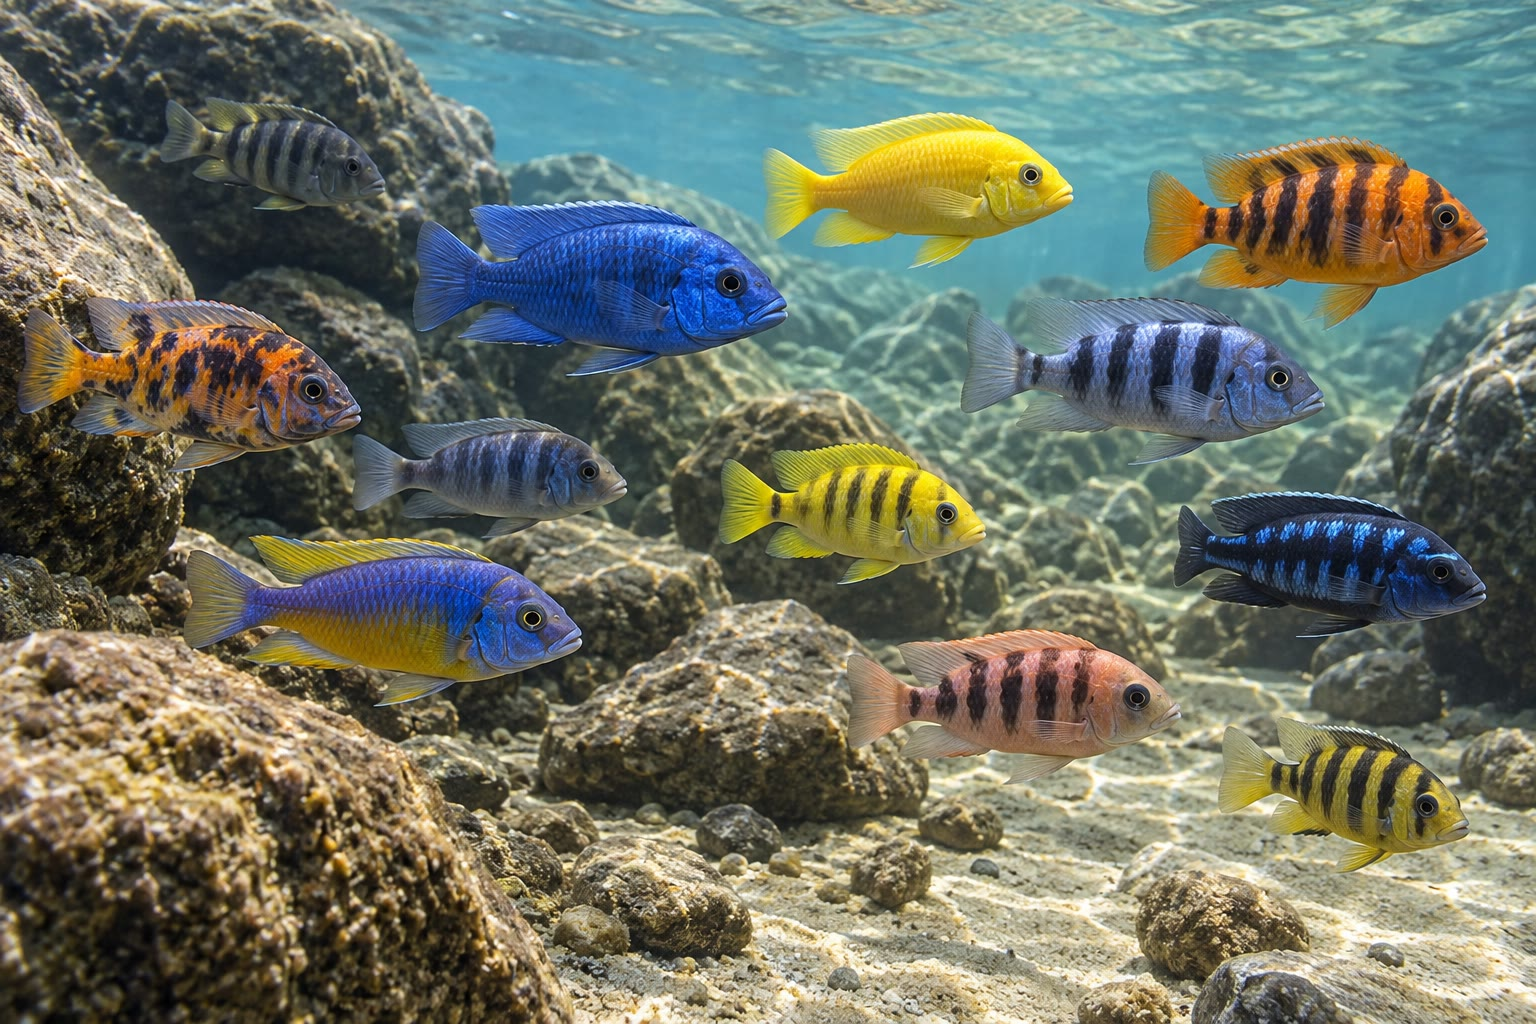
\includegraphics[width=0.6\linewidth]{images/book5/ai/b5-25-cichlids.jpg}

{\small بلطي بحيرة أفريقية: مئات الأنواع في بضعة آلاف من
السنين، وفروقها مسحوبة في معظمها من تباين كانت أسلافها
المشتركة تحمله أصلًا.}
\end{omfigure}

\begin{remark}[المصادفة خطَّ أساس]\label{rem:b3:molecular-evolution:remark}
\omterm{thm:b3:molecular-evolution:neutral}{النظرية المحايدة} ليست دعوى بأن الانتخاب غير مهم؛ بل هي بيان
لما يحدث حين يغيب الانتخاب، دقيق بما يكفي لأن يُختبر في
مواجهته. فلأن المعدل المحايد هو معدل الطفر، يقيس التباعد
الزمن؛ ولأن التغيّر المحايد يملأ المواقع التي يتركها الانتخاب
حرة، يقيس $\omega$ القيد؛ ولأن السلالات المحايدة تتلاقى
بمعدل معلوم، يقيس خلافُ أشجار المورّثات حجمَ جمهرات لم يرها
أحد. فالانتخاب عندئذ ما يبقى بعد طرح المصادفة --- مورّثة
عندها $\omega$ فوق الواحد، أو كسحة أفرغت التباين من منطقة، أو
شجرة تخالف في اتجاه لا يفسره الانجراف. ومانع تجمد سمكة
الجليد الأنتاركتيكية، وليزوزيم معدة المجترّ، وأوبسين الرئيسي
الثالث هي الاستثناءات المكتشفة بهذا الطريق، وكل واحد منها
قصة مورّثة منسوخة وعمل جديد. وأما سائر الجينوم فساعة.
\end{remark}

\section{تمارين}

\begin{exercise}[$\star$]\label{exo:b3:molecular-evolution:1}
اذكر \omterm{thm:b3:molecular-evolution:neutral}{معدل الاستبدال} المحايد واشرح بالكلام لماذا لا يتوقف على
حجم الجمهرة.
\end{exercise}

\begin{exercise}[$\star$]\label{exo:b3:molecular-evolution:2}
عرّف النظيرة المباشرة، والنظيرة المتضاعفة، \omterm{def:b3:molecular-evolution:duplication}{والمورّثة الكاذبة}،
مع مثال واحد من عائلة الغلوبين لكل منها.
\end{exercise}

\begin{exercise}[$\star$]\label{exo:b3:molecular-evolution:3}
ماذا تقيس $\omega = d_{N}/d_{S}$؟ فسّر $\omega = 0.02$،
و$\omega = 1.0$، و$\omega = 2.5$، وسمّ مورّثة من كل صنف.
\end{exercise}

\begin{exercise}[$\star$]\label{exo:b3:molecular-evolution:4}
لماذا استنتج كيمورا أن معظم الاستبدالات محايدة؟ أعد صوغ
الحجة بالأرقام في مطلع الفصل.
\end{exercise}

\begin{exercise}[$\star\star$]\label{exo:b3:molecular-evolution:5}
$N = 5000$. احسب احتمال تثبّت طفرة جديدة عند $s
= 0$، و$s = 0.001$، و$s = 0.01$، و$s = -0.001$، بصيغة كيمورا،
وعلّق على أيها محايد فعليًا.
\end{exercise}

\begin{exercise}[$\star\star$]\label{exo:b3:molecular-evolution:6}
يختلف نوعان في \qty{12}{\%} من مواقع مورّثة معدلها المحايد
\qty{2e-9}{} لكل موقع في السنة. قدّر زمن تباعدهما مع تصحيح
جوكس--كانتور وبدونه. وعند أي فرق خام يبلغ التصحيح عاملًا قدره اثنان؟
\end{exercise}

\begin{exercise}[$\star\star$]\label{exo:b3:molecular-evolution:7}
مورّثة من 300 رامزة فيها 700 موقع غير مرادف و200 موقع مرادف.
وهي تُظهر بين نوعين 7 فروق غير مرادفة و10 فروق مرادفة. احسب
$p_{N}$ و$p_{S}$ و$\omega$ (بلا تصحيح). فأي نظام انتخابي؟ وماذا
لو كان العددان 35 و10؟
\end{exercise}

\begin{exercise}[$\star\star$]\label{exo:b3:molecular-evolution:8}
تختلف المتواليات المحايدة عند الإنسان والشمبانزي في
\qty{1.2}{\%}؛ وكان الانفصال قبل \qty{6.5}{Myr}، وزمن الجيل
\qty{25}{yr}. قدّر معدل الطفر لكل موقع في الجيل، وعدد الطفرات
الجديدة في جينوم ثنائي الصيغة من $6\times 10^{9}$ أساس في كل جيل.
\end{exercise}

\begin{exercise}[$\star\star$]\label{exo:b3:molecular-evolution:9}
عند $N = \num{50000}$ و$T = \num{100000}$ جيل بين
الانفصالين، احسب نسبة أشجار المورّثات المخالِفة لشجرة
الأنواع عند الإنسان والشمبانزي والغوريلا. وأي $T$ يجعلها
\qty{10}{\%}؟
\end{exercise}

\begin{exercise}[$\star\star\star$]\label{exo:b3:molecular-evolution:10}
بيّن أن صيغة كيمورا تؤول إلى $1/2N$ حين $s \to 0$ وإلى $2s$
عند $4Ns \gg 1$، وأنها عند $s < 0$ مع $4N|s| \gg 1$ تسلك سلوك
$2|s|\,\mathrm{e}^{-4N|s|}$. ومن ثم قدّر كم يجب أن تكون طفرة
ضارة، في جمهرة من $10^{4}$، ليهبط احتمال تثبّتها مئة ضعف دون
المحايد.
\end{exercise}

\begin{exercise}[$\star\star\star$]\label{exo:b3:molecular-evolution:11}
اختبار معدل نسبي: مجموعة خارجية $O$ على مسافة مصحَّحة $0.30$
من الفأر و$0.24$ من الإنسان، والفأر والإنسان متباعدان $0.20$. احسب طولي فرعي
الفأر والإنسان منذ انفصالهما (بافتراض أن نقطة الانفصال
متساوية البعد عن $O$ على المسارين)، ونسبتهما. ومع جيل فأر
قدره \qty{0.5}{yr} وجيل إنسان قدره \qty{25}{yr}، بماذا كانت
ستتنبأ ساعة صارمة في كل جيل بالنسبة، وماذا تقول الملاحظة عن
معدلات الطفر في الجيل؟
\end{exercise}

\begin{exercise}[$\star\star\star$]\label{exo:b3:molecular-evolution:12}
تتحرر مورّثة مضاعَفة من القيد ($\omega = 1$) عند معدل محايد
$k = \qty{2e-9}{}$ لكل موقع في السنة. ففي متوالية مرمِّزة من
1000 أساس، كم سنة تقريبًا حتى تُتوقَّع أول رامزة وقف أو
انزياح إطار (بافتراض أن نحو \qty{4}{\%} من الطفرات النقطية
العشوائية في متوالية مرمِّزة تصنع رامزة وقف، وبإهمال الإدخالات
والحذوف)؟ وقارن ذلك بالزمن المتاح للانتخاب ليجد وظيفة جديدة،
واشرح لماذا تموت معظم النسخ المضاعَفة.
\end{exercise}

\section{مسألة: معدل التغيّر}

\begin{problem}[{مسألة نهاية الأسبوع --- تاريخ جينوم بالأرقام:
معدل الطفر من تباعد الإنسان والشمبانزي، وحمل الاستبدال عند
كيمورا، وحظوظ تثبّت الطفرات المنتخَبة، ونسبة $\omega$ لمورّثة
من عدّ الرامزات، والساعة مقروءةً لتضاعف، وخلاف أشجار
المورّثات بين القردة العليا، وتُختم بمعدل الطفر، وبنسبة
$\omega$ للمورّثة، وبنسبة الأشجار المخالِفة}]
\label{pb:b3:molecular-evolution:1}
المعطيات: التباعد المحايد بين الإنسان والشمبانزي $d = 0.012$؛
والانفصال قبل \qty{6.5}{Myr}؛ والجيل \qty{25}{yr}؛ والجينوم
الثنائي الصيغة $6\times
10^{9}$ أساس، و\qty{1.5}{\%} منه مرمِّز. والجمهرة السلفية $N =
\num{50000}$. والمورّثة: 400 رامزة، و920 موقعًا غير مرادف و280
موقعًا مرادفًا؛ وفروق الإنسان والفأر 46 غير مرادف و84 مرادفًا.
وانفصال الإنسان والفأر \qty{90}{Myr}. والغلوبين: يختلف $\alpha$ و$\beta$ في
\qty{55}{\%} من مواقع الأحماض الأمينية (خامًا)؛ ومعدل الهيموغلوبين \num{1e-9} لكل
موقع في السنة. والقردة: $T$ بين انفصالي الغوريلا والشمبانزي
\num{80000} جيل. وحدّ هالدين: استبدال منتخَب واحد لكل
300 جيل.

\medskip
\noindent\textbf{الجزء الأول --- المعدل.}
\begin{enumerate}
  \item من $d = 2kT$، احسب $k$ لكل موقع في السنة، ثم $\mu$ لكل
        موقع في الجيل.
  \item الطفرات الجديدة في الجينوم الثنائي الصيغة في الجيل،
        وكم منها يقع في متوالية مرمِّزة.
  \item الاستبدالات المثبَّتة في الجيل في الجينوم كله عند
        المعدل المحايد (فالجمهرة تثبّت $\mu$ لكل موقع في
        الجيل). قارن ذلك بحدّ هالدين واستخرج نتيجة كيمورا.
  \item في جمهرة من $N = \num{50000}$، كم طفرة محايدة جديدة
        تنشأ لكل موقع في الجيل في الجمهرة كلها،
        وأي نسبة منها ستتثبت يومًا؟
  \item كم تستغرق طفرة محايدة مقدَّر لها التثبّت،
        بالأجيال وبالسنين؟ قارن ذلك بالزمن منذ انفصال
        الإنسان والشمبانزي.
  \item اشرح لماذا يقيس التباعد بين نوعين، رغم السؤال~5،
        الزمن منذ انفصالهما لا الزمن منذ تثبّت أليلاتهما.
\end{enumerate}

\medskip
\noindent\textbf{الجزء الثاني --- حظوظ الانتخاب.}
\begin{enumerate}[resume]
  \item احتمال تثبّت طفرة محايدة عند $N = \num{50000}$،
        وطفرة عند $s = 0.001$، و$s = 0.01$، و$s = 0.1$.
  \item عند أي $s$ يكون $4Ns = 1$؟ فسّر الحد.
  \item طفرة ضارة عند $s = -0.001$: احتمال تثبّتها
        نسبةً إلى المحايدة. وعند $s = -10^{-5}$؟
  \item إذا كانت نسبة $10^{-5}$ من الطفرات الجديدة في مورّثة
        نافعةً عند $s = 0.01$ والباقي محايدًا، فأي نسبة من
        الاستبدالات في تلك المورّثة تكيّفية؟ علّق على قلة
        ظهور الانتخاب في المتوالية حتى حين يعمل.
  \item احسب $p_{N}$ و$p_{S}$ لمورّثة الإنسان والفأر، وصحّح
        كلًّا منهما بجوكس--كانتور، وأعطِ $\omega$.
  \item فسّر $\omega$؛ وقدّر المعدل المحايد الذي تقتضيه
        $d_{S}$ للمورّثة (لكل موقع في السنة) مستعملًا زمن
        الانفصال. وهل يتسق ذلك مع السؤال~1؟
\end{enumerate}

\medskip
\noindent\textbf{الجزء الثالث --- الساعات والنسخ.}
\begin{enumerate}[resume]
  \item صحّح فرق الغلوبين $\alpha$--$\beta$ للإصابات المتعددة
        (استعمل $d = -\ln(1 - p)$، وهي صورة البروتين ذات
        الحالات الكثيرة)، وأرّخ التضاعف بمعدل الهيموغلوبين.
  \item يقع التاريخ قرب أصل الفقاريات ذوات الفكوك
        (\qtyrange{450}{500}{Myr}). فماذا يتيح وجود سلسلتي
        $\alpha$ و$\beta$ منفصلتين مما لا تتيحه سلسلة واحدة؟
  \item تتغير الببتيدات الليفينية عند $8\times 10^{-9}$ لكل موقع في
        السنة. ونوعان انفصلا قبل \qty{40}{Myr}: فما الفرق الخام
        المتوقع؟ ولماذا يكون هذا البروتين عديم الفائدة لتأريخ
        انفصالات عمرها \qty{500}{Myr}؟
  \item يتغير \omterm{def:b3:chromatin-epigenetics:nucleosome}{الهستون} H4 عند $10^{-11}$: فكم استبدالًا في 100
        موقع على مدى \qty{1000}{Myr}؟ ولماذا يكون عديم الفائدة
        لتأريخ الانفصالات الحديثة؟
  \item تنجرف مورّثة مضاعَفة عند $\omega = 1$ من لحظة
        التضاعف. فإذا صنعت \qty{4}{\%} من الاستبدالات في
        المتوالية المرمِّزة رامزات وقف، وكان في المورّثة 1200
        موقع عند معدل $2\times
        10^{-9}$ لكل موقع في السنة، قدّر الزمن المتوقع حتى
        أول رامزة وقف.
  \item لماذا يعطي تضاعف الجينوم الكامل النسخَ المضاعَفة حظًا
        أفضل في البقاء من تضاعف ترادفي مفرد؟
\end{enumerate}

\medskip
\noindent\textbf{الجزء الرابع --- أشجار داخل أشجار.}
\begin{enumerate}[resume]
  \item احتمال أن تخفق سلالة إنسانية وسلالة شمبانزية في
        التلاقي في \num{80000} جيل قبل انفصال الغوريلا.
  \item نسبة أشجار المورّثات المخالِفة لشجرة الأنواع.
        والمرصود: نحو \qty{30}{\%}. فهل يتسق؟
  \item من الأشجار المخالِفة، أي نسبة تضم الإنسان إلى
        الغوريلا، وأي نسبة تضم الشمبانزي إلى الغوريلا؟ وبماذا
        كان سيدل خروج قوي عن التساوي؟
  \item لو كانت الجمهرة السلفية $N = \num{10000}$، فأي نسبة
        مخالِفة كنت ستتوقع؟ وبماذا تدل النسبة المرصودة إذن
        على أعداد أسلافنا؟
  \item لماذا يعطي جمع ألف مورّثة في \omterm{def:b3:bioinformatics:alignment}{محاذاة} واحدة شجرةً واثقة
        لكنها قد تكون خاطئة، وماذا تفعل طريقة التلاقي بدل ذلك؟
  \item يبلغ DNA النياندرتالي في البشر غير الأفارقة نحو
        \qty{2}{\%} وتضم الأشجار الحاملة له بعض الأوروبيين إلى
        النياندرتاليين أكثر مما تضم الأفارقة. فلماذا لا يكون
        ذلك فرزًا سلاليًا غير تام؟
  \item لخّص: قيمة $\mu$ (السؤال~1)، ونسبة $\omega$ للمورّثة
        (السؤال~11)، ونسبة الأشجار المخالِفة (السؤال~20).
\end{enumerate}
\end{problem}
